\chapter{Introduction}
\label{cha:introduction}

\section{Motivation}
\emph{Minimally Invasive Surgery (MIS)} has a considerable impact on modern surgical practice:
By inserting specialized instruments (see figure~\ref{img:lap_instruments}) and a laparoscope through small access ports, the surgeon can operate on the internal anatomy under direct video observation of the surgical site without making large incisions (see figure~\ref{img:laparoscopy}). MIS performed in the abdomen and pelvis is also referred to as \emph{laparoscopic surgery}.~\cite{advances_minimal_surgery2002darzi} 

\begin{figure}
\centering
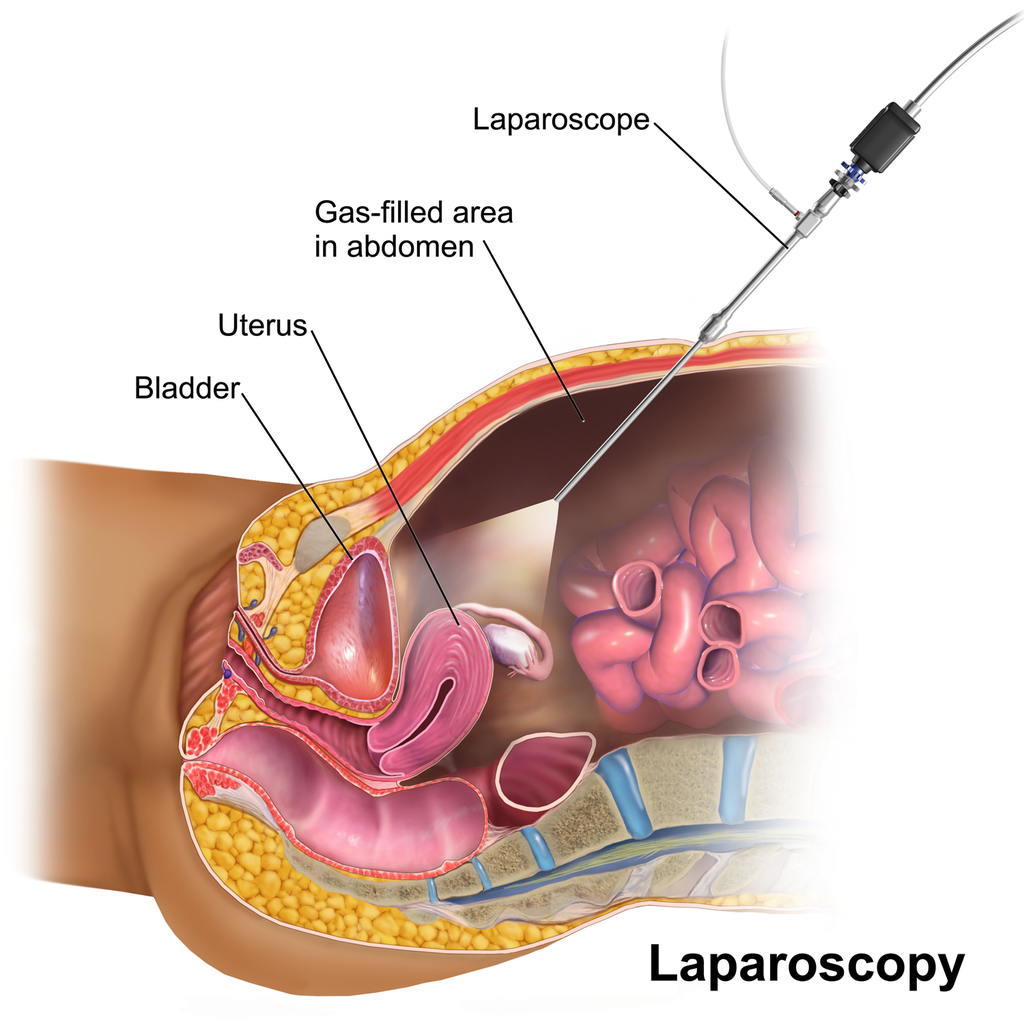
\includegraphics[width=0.45\textwidth]{images/laparoscopy_example_graphic.png}
\caption[Example MIS]{Illustration of MIS by Blausen et al.~\cite{laparosc_image2014blausen} The surgeon is getting the view of the operation scene by the laparoscope as real-time video.}
\label{img:laparoscopy}
\end{figure}

\begin{figure}
\centering
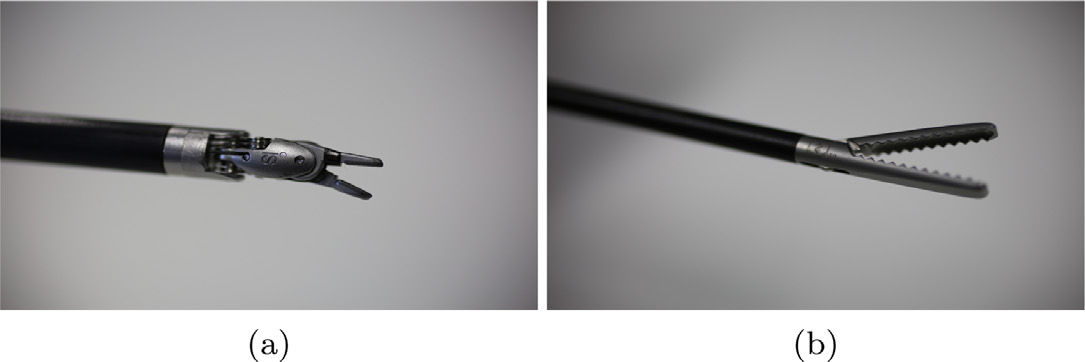
\includegraphics[width=0.5\textwidth]{images/laparoscopic_instruments.png}
\caption[Example MIS surgical instruments]{Examples of different MIS instruments: (a)~Da Vinci~\cite{da_vinci_localization2005Leven} articulated robotic instrument, (b)~rigid laparoscopic instrument~\cite{vision_based_surg_tool_det2017bouget}.}
\label{img:lap_instruments}
\end{figure}

Because the surgical instruments required for this technique are smaller and the advanced instrument 
design improves tissue manipulation, the surgical trauma for the patient after surgery is reduced~\cite{vision_based_surg_tool_det2017bouget}. 
Rutherford et al.~\cite{laparoscopic_adrenalectomy1996rutherford} showed in a laparoscopic adrenalectomy study that the postoperative inpatient stay was decreased from 9.8 to 5.1 days in comparison to the commonly known open surgery approach. Lacy et al.~\cite{laparoscp2002lacy} showed in a study regarding colorectoral cancer operation that patients treated with MIS recovered faster, had shorter hospital stays, and higher probability of cancer-related survival.

%\emph{Computer assisted intervention (CAI)} systems are used to gain information before and and during the surgery process with the aim to overcome these challenges.~\cite{vision_based_surg_tool_det2017bouget}

Before it is possible to perform MIS, the surgeons and the rest of the clinical team have to be trained to operate with MIS instruments. There are several challenges compared to open surgical approaches~\cite{haptic_feedback_surgery2009vanderMeijden}: 
The sense of touch for the surgeon is reduced and the view of the surgery is restricted by the endoscopic camera. It is also important to integrate image guidance to protect critical structures and help the surgeon to locate anatomical targets. Real-time knowledge of the position of the instruments within the surgical field of view is one of the main goals to improve MIS.~\cite{detect_instruments_mis2013allan} 

The following approaches are currently used to overcome the instrument localization challenge in MIS:
Electromagnetic tracking, which is realised by attaching an electromagnetic device to the instrument~\cite{electromagnetic_tracking2016lahanas}.
Optical localizers, where markers are applied to the surgical instrument and an additional external camera is used to recognize these markers and calculate the position of the instrument. This is the most widespread method in clinical use~\cite{optical_localizer_instr2010elfring}.
Other common methods are gaining positional information out of robotic surgery systems~\cite{da_vinci_localization2005Leven}, 
ultrasound-based methods~\cite{ultrasound_localization2009Hu}, and localization based on the endoscopic video used by the surgeon to operate~\cite{Laina2017}.

\section{Goals}
Image-based localization approaches are highly attractive because they do not require modification of the instrument design or the operating room, like for example electromagnetic tracking or optical localizers: 
The position and motion information is obtained directly from endoscopic camera used by the surgeon to operate. This is also the method with the lowest expenses.~\cite{vision_based_surg_tool_det2017bouget}
The aim is therefore to develop an image-based localization method for assistance and improvement of MIS.

% Input to proposed methods:
The input to the segmentation and localization methods proposed in this work are images out of an endoscopic video. The images contain surgical instruments.
%Def. Segmentation:
Segmentation means partitioning the input image into instrument part and background part. The partitioned image contains high pixel values where the instrument is located and low pixel values where the background is located.
% Def. Localization: 
Localization means extracting the pixel position of specific instrument landmarks out of the input image. In this work, the center point of the shown instruments is located.

Convolutional Neural Networks currently provide the best solutions for image segmentation~\cite{miccai15_results2018bodenstedt,long2015_FCNs}. This image segmentation task can be enhanced to localization of surgical instruments in images, as recently shown by Laina et al.~\cite{Laina2017}. 
In this work, the segmentation CNN proposed by Shvets et al.~\cite{Shvets2018} is extended with the aim to solve the localization task based on previously learned segmentation information.

%For the segmentation task, the prediction of the network divides the input image into instrument and background. The prediction is a greyscale image, where a high pixel value indicates a high probability that a part of the instrument is located at this position.  A low pixel value indicates a high probability that the background is shown at this pixel position. 
%
%For the localization task, the prediction of the network is a greyscale image that contains the highest pixel values near the instrument center point position.
%A low pixel value in the prediction indicates a high probability that this pixel is part of the background. In a postprocessing step, the exact position of the instrument is extracted out of the prediction image.